\section{Software} \label{sec:software}
Einleitung in unsere Software, MVC-Aufbau
\begin{figure}[H]
	\begin{minipage}[h]{0.45\linewidth}
		\centering
		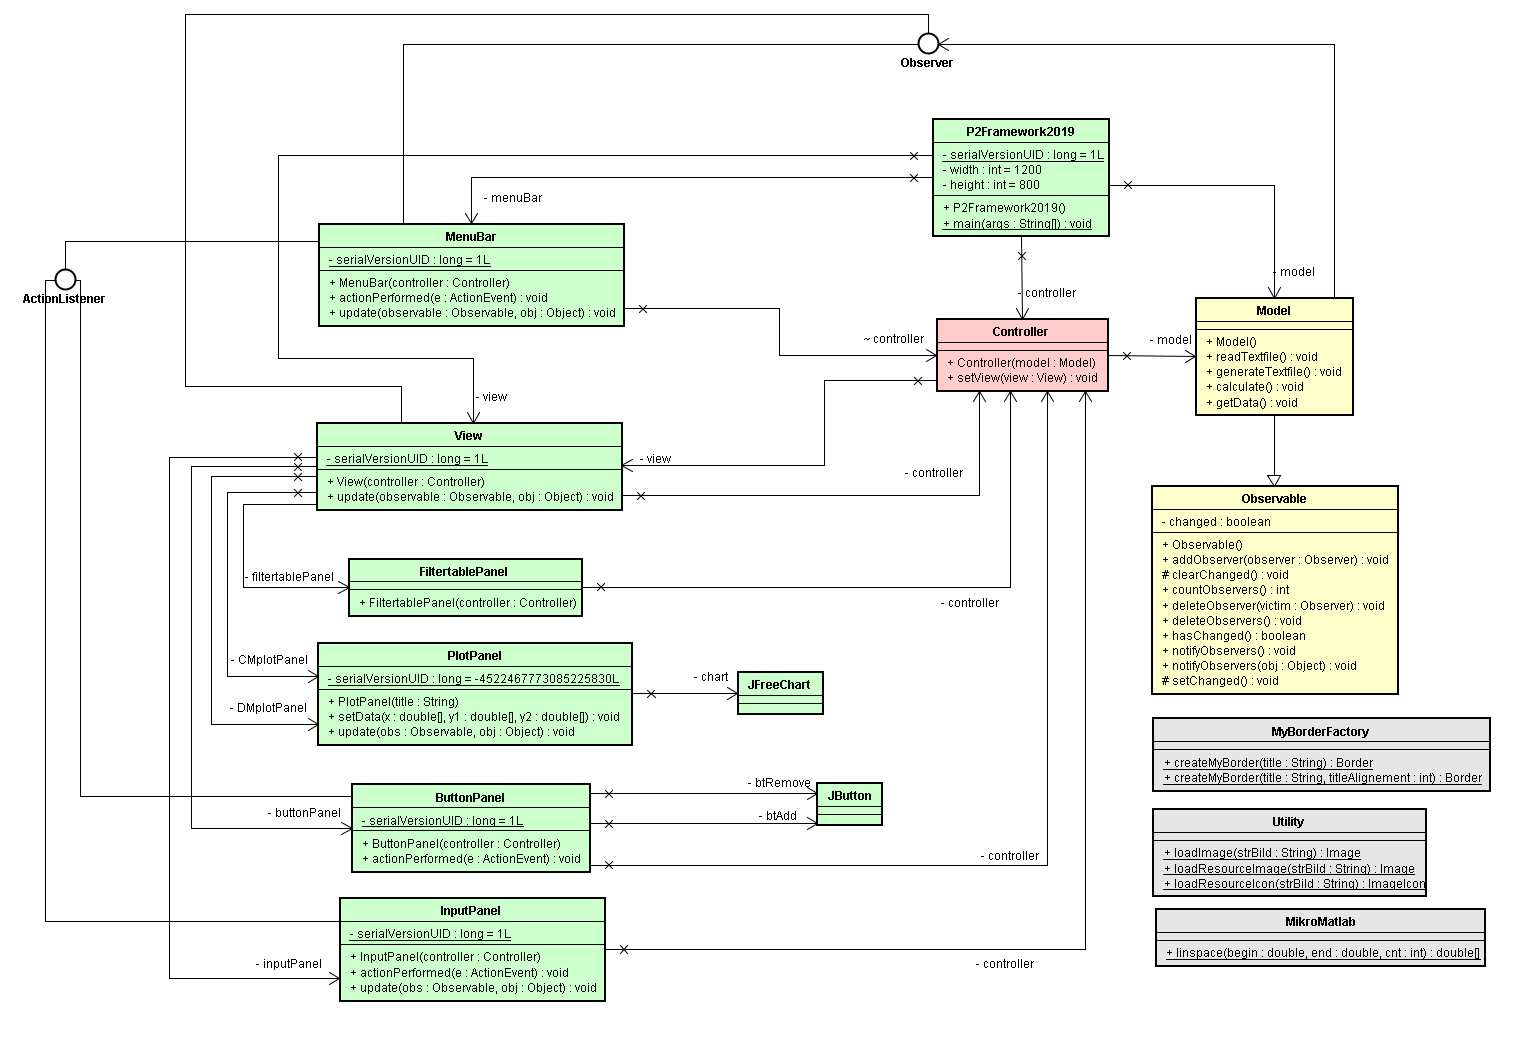
\includegraphics[width = 18cm]{Klassendiagramm.png}
		\label{fig:piImpedance}
		\caption{Klassendiagramm \cite{wtf}}
	\end{minipage}
\end{figure}

\subsection{Ermittlung der Schaltung} \label{subsec:ermittlung}
Aufbrechen der Schaltung, beschrieb der Klassen und Methoden des Models

\begin{figure}[H]
	\begin{minipage}[h]{0.45\linewidth}
		\centering
		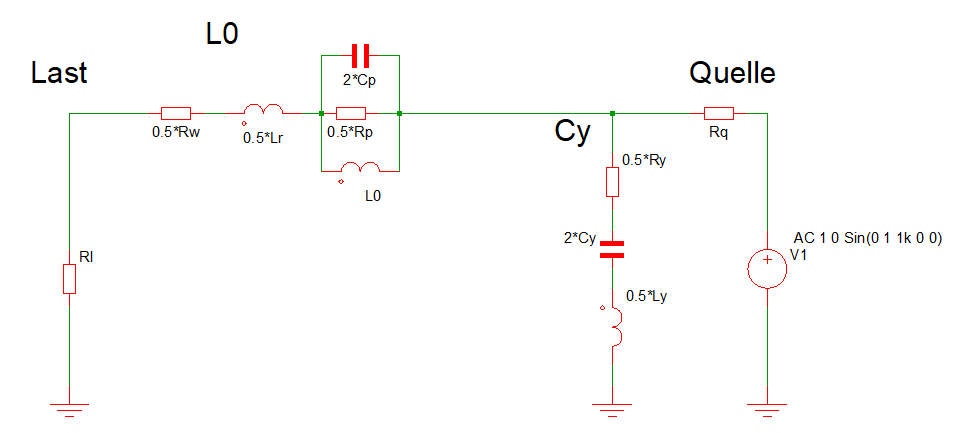
\includegraphics[width = 6cm]{EMI_CM.png}
		\label{fig:piImpedance}
		\caption{Vereinfachte \cite{CM_Schaltung}}
	\end{minipage}
\end{figure}

\begin{figure}[H]
	\begin{minipage}[h]{0.45\linewidth}
		\centering
		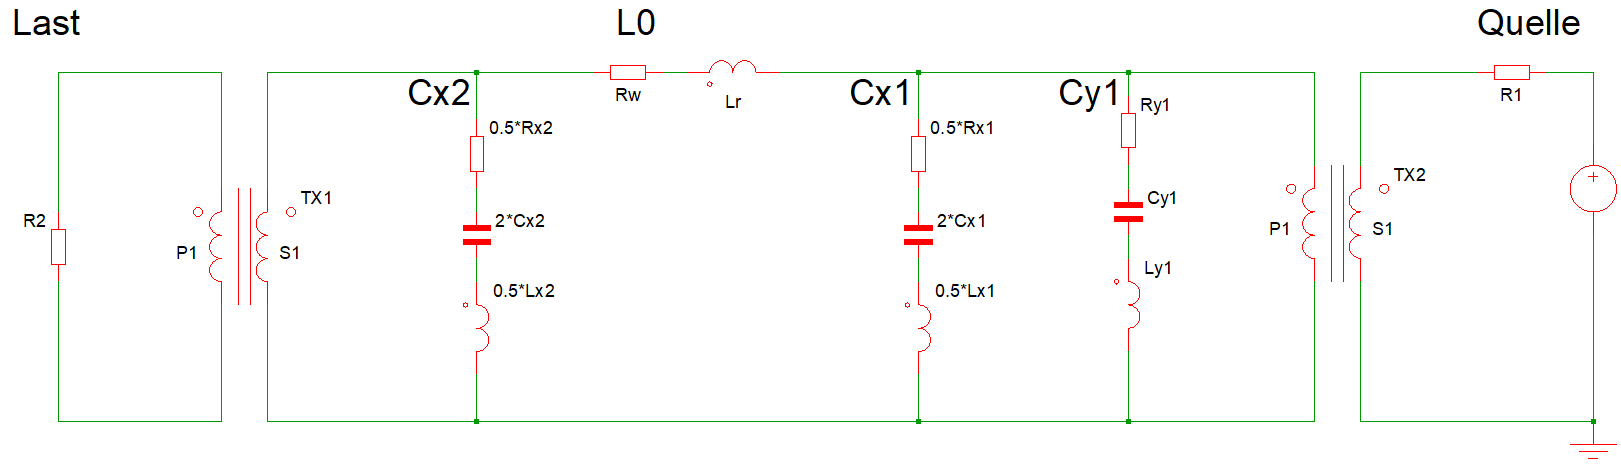
\includegraphics[width = 6cm]{EMI_DM.png}
		\label{fig:piImpedance}
		\caption{Vereinfachte \cite{DM-Schaltung}}
	\end{minipage}
\end{figure}


\subsection{Benutzeroberfläche} \label{subsec:benutzeroberflaeche}
Aufbau unserer GUI zeigen, Datenverarbeitung aufzeigen und Zusammenspiel der Panels erklären

Danach subsub's der einzelnen Panels um deren Funktionen zu zeigen


\subsubsection{Plotpanel} \label{subsubsec:plotpanel}



\subsubsection{Menu}\label{subsubsec:menu}


\subsubsection{Inputpanel} \label{subsubsec:inputpanel}


\subsubsection{Filtertabelle} \label{subsubsec:filtertabelle}





